\subsection{UML Diagramme}
\label{sec:UMLDiagramme}

Quelle: Oose.de - Notationsübersicht UML \cite{UMLNotationsuebersicht} \& IHK Belegsatz

\subsubsection{Klassendiagramm}
\label{sec:Klassendiagramm}

\begin{center}
	\begin{tikzpicture}[align=center]
		
		\draw (0,3) node[minimum height=1.5cm, minimum width=3cm, draw](klasse) {Klasse};
		\node[minimum height=1.5cm, minimum width=3cm, draw, font=\itshape, right=1.5cm of klasse](abstrKlasse) {Abstrakte\\Klasse};
		
		\node [minimum height=1.5cm, minimum width=3cm, draw, below=1cm of klasse] {Aktive\\Klasse};
		\node [minimum height=1.5cm, minimum width=2.8cm, draw, below=1cm of klasse] {};
		
		\draw (3,-0.3) -- (6,-0.3) -- (6,0.8) -- (5.2,1.2) node[below left=15pt and 5pt]{Notiz} -- (3,1.2) -- (3,-0.3);
		\draw (5.2,1.2) -- (5.2,0.8) -- (6,0.8);
		\draw [dashed] (3,0.45) -- (2.2,0.45);
		
		\draw (8,0) rectangle (14,4); 
		
		\node at (9.4,0.4){attribut = wert};
		\node at (11,0.8){<<Stereotyp1>>};
		\draw (8,1.2) -- (14,1.2);
		\node at (9.1,1.6) {operation()};
		\draw (8,2) -- (14,2);
		\node at (8.8,2.4) {attribut};
		\draw (8,2.8) -- (14,2.8);
		\node at (11,3.4) {<<Stereotyp1, Stereotyp2>>\\Paket::Klasse};
	\end{tikzpicture}
\end{center}

Sichtbarkeit:
\begin{multicols}{2}
	\begin{itemize}
		\item Öffentlich (+)
		\item Privat (-)
		\item Geschützt (\#)
		\item Paket (\textasciitilde)
		\item Abgeleitet (/)
		\item Statisch (unterstrichen)
	\end{itemize}
	\columnbreak
	\textbf{Syntax für Attribute:}\\
	Sichtbarkeit Attributname: Typ \{Eigenschaften\}
	
	\textbf{Syntax für Methoden:}\\
	Sichtbarkeit Methodenname(parpameter1: Typ, ...): Rückgabewert \{Eigenschaften\}
	
	\textbf{Eigenschaften:}\\
	\{static,final, ...\}
\end{multicols}

\vspace{2em}

\begin{multicols}{2}
	\begin{center}
		\begin{tikzpicture}[align=center, node distance=3.5cm]
			\node[minimum height=1cm, minimum width=2cm, draw](vererbungklasse1){Klasse 1};
			\node[minimum height=1cm, minimum width=2cm, draw, right=of vererbungklasse1](vererbungklasse2){Klasse 2};
			\draw[-{Triangle[open]}, thick] (vererbungklasse1) -- (vererbungklasse2) node[pos=.5,above]{Vererbung};
			
			\node[minimum height=1cm, minimum width=2cm, draw, below=1cm of vererbungklasse1](assoziationklasse1){Klasse 1};
			\node[minimum height=1cm, minimum width=2cm, draw, below=1cm of vererbungklasse2](assoziationklasse2){Klasse 2};
			\draw[thick] (assoziationklasse1) -- (assoziationklasse2) node[pos=.5,above]{Assoziation};
			
			\node[minimum height=1cm, minimum width=2cm, draw, below=1cm of assoziationklasse1](gerichteteassoziationklasse1){Klasse 1};
			\node[minimum height=1cm, minimum width=2cm, draw, below=1cm of assoziationklasse2](gerichteteassoziationklasse2){Klasse 2};
			\draw[{-to}, thick] (gerichteteassoziationklasse1) -- (gerichteteassoziationklasse2) node[pos=.5,above]{gerichtete\\Assoziation};
		\end{tikzpicture}
	\end{center}
	
	\begin{center}
		\begin{tikzpicture}[align=center, node distance=3.5cm]
			\node[minimum height=1cm, minimum width=2cm, draw](realisierungklasse1){Klasse 1};
			\node[minimum height=1cm, minimum width=2cm, draw, right=of realisierungklasse1](realisierungklasse2){Klasse 2};
			\draw[-{Triangle[open]}, thick, dashed] (realisierungklasse1) -- (realisierungklasse2) node[pos=.5,above]{Implementierung};
			
			\node[minimum height=1cm, minimum width=2cm, draw, below=1cm of realisierungklasse1](abhaengigeklasse){Abhängige\\Klasse};
			\node[minimum height=1cm, minimum width=2cm, draw, below=1cm of realisierungklasse2](unabhaenigeKlasse){Unabhängige\\Klasse};
			\draw[->, thick, dashed] (abhaengigeklasse) -- (unabhaenigeKlasse) node[pos=.5,above]{Abhängigkeit};
		\end{tikzpicture}
	\end{center}
\end{multicols}

\newpage

\begin{multicols}{2}
	\begin{center}
		\begin{tikzpicture}[align=center, node distance=2.5cm]
			\node[minimum height=1cm, minimum width=2cm, draw](attributierteklasse1){Klasse 1};
			\node[minimum height=1cm, minimum width=2cm, draw, right=of attributierteklasse1](attributierteklasse2){Klasse 2};
			\draw[thick] (attributierteklasse1) -- (attributierteklasse2) node[pos=.5,above]{Attributierte\\Assoziation};
			\node[minimum height=1cm, minimum width=2cm, draw,below right=1cm and 0cm of attributierteklasse1](assoziationsklasse){Assoziations-\\Klasse};
			\draw[thick, dashed] (assoziationsklasse) -- (2.22,0);
			
			\node[minimum height=1cm, minimum width=2cm, draw, below=4cm of attributierteklasse1](mehrGliedrAssoKlasse1){Klasse 1};
			\node[minimum height=1cm, minimum width=2cm, draw, below=4cm of attributierteklasse2](mehrGliedrAssoKlasse2){Klasse 2};
			\node[minimum height=1cm, minimum width=2cm, draw, diamond, scale=0.5](dia) at ($(mehrGliedrAssoKlasse1)!0.5!(mehrGliedrAssoKlasse2)$) {};
			\node[above=0.2cm of dia]{Mehrgliedrige\\Assoziation};
			\draw[thick] (mehrGliedrAssoKlasse1) -- (dia);
			\draw[thick] (dia) -- (mehrGliedrAssoKlasse2);
			\node[minimum height=1cm, minimum width=2cm, draw, below right=0.5cm and 0.25cm of mehrGliedrAssoKlasse1](mehrGliedrAssoKlasse3){Klasse 3};
			\draw[thick] (mehrGliedrAssoKlasse3) -- (dia);
		\end{tikzpicture}
	\end{center}
	
	\begin{center}
		\begin{tikzpicture}[align=center, node distance=2.5cm]
			\node[minimum height=1cm, minimum width=2cm, draw, below=3cm of attributierteklasse2](Teil){Teil};
			\node[minimum height=1cm, minimum width=2cm, draw, below=1cm of Teil, below=0.5cm of Teil](existAbhTeil){Existenz-\\abhängiges Teil};
			\node[minimum height=3cm, minimum width=2cm, draw, below left=-1.1cm and 2.5cm of Teil](ganzesAggKomp){Ganzes};
			\draw[-{Diamond[open]},thick] (Teil) -- (ganzesAggKomp) node[pos=.5,above,rotate=12]{Aggregation};
			\draw[-Diamond,thick] (existAbhTeil) -- (ganzesAggKomp) node[pos=.5,below,rotate=-10]{Komposition};
		\end{tikzpicture}
	\end{center}
\end{multicols}

%\begin{minipage}[c]{0.65\textwidth}
%	\begin{itemize}
%		\item \textbf{Vererbung}: Prozess, bei dem eine Unterklasse die Eigenschaften einer Oberklasse übernimmt, wird auch als Generalisierung bezeichnet. Dargestellt durch eine gerade Verbindungslinie mit geschlossener Pfeilspitze, die auf die Oberklasse zeigt.
%	\end{itemize}
%\end{minipage}
%\hfill
%\begin{minipage}[c]{0.25\textwidth}
%	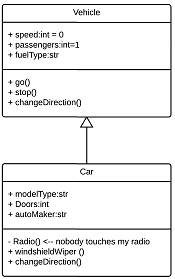
\includegraphics[scale=.7]{Bilder/Klassendiagramm/InteraktionVererbung.png}
%\end{minipage}

\subsubsection{Use-Case-Diagramm (Anwendungsfalldiagramm)}
\label{sec:UseCaseDiagramm}

Quelle: Ionos \cite{IonosUseCase}

\begin{center}
	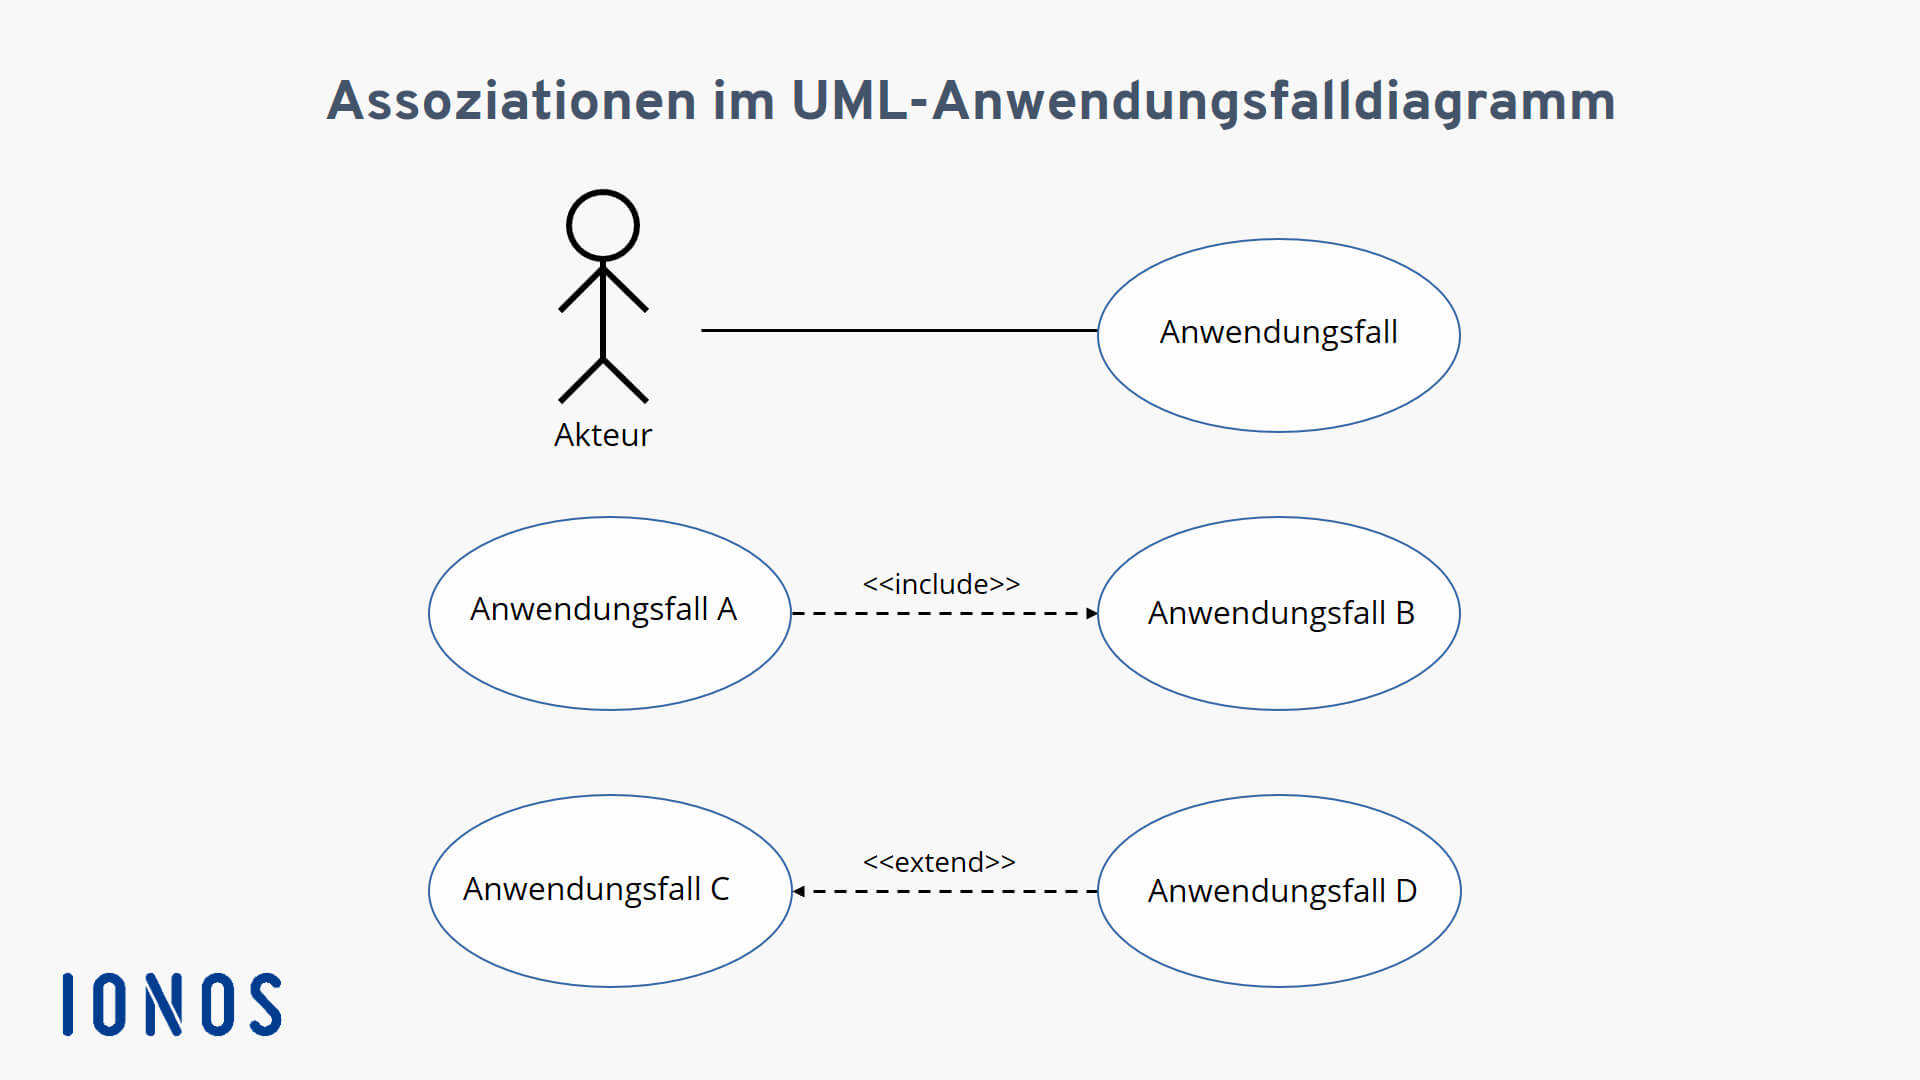
\includegraphics[scale=.25]{Bilder/UseCaseDiagram.png}
	
	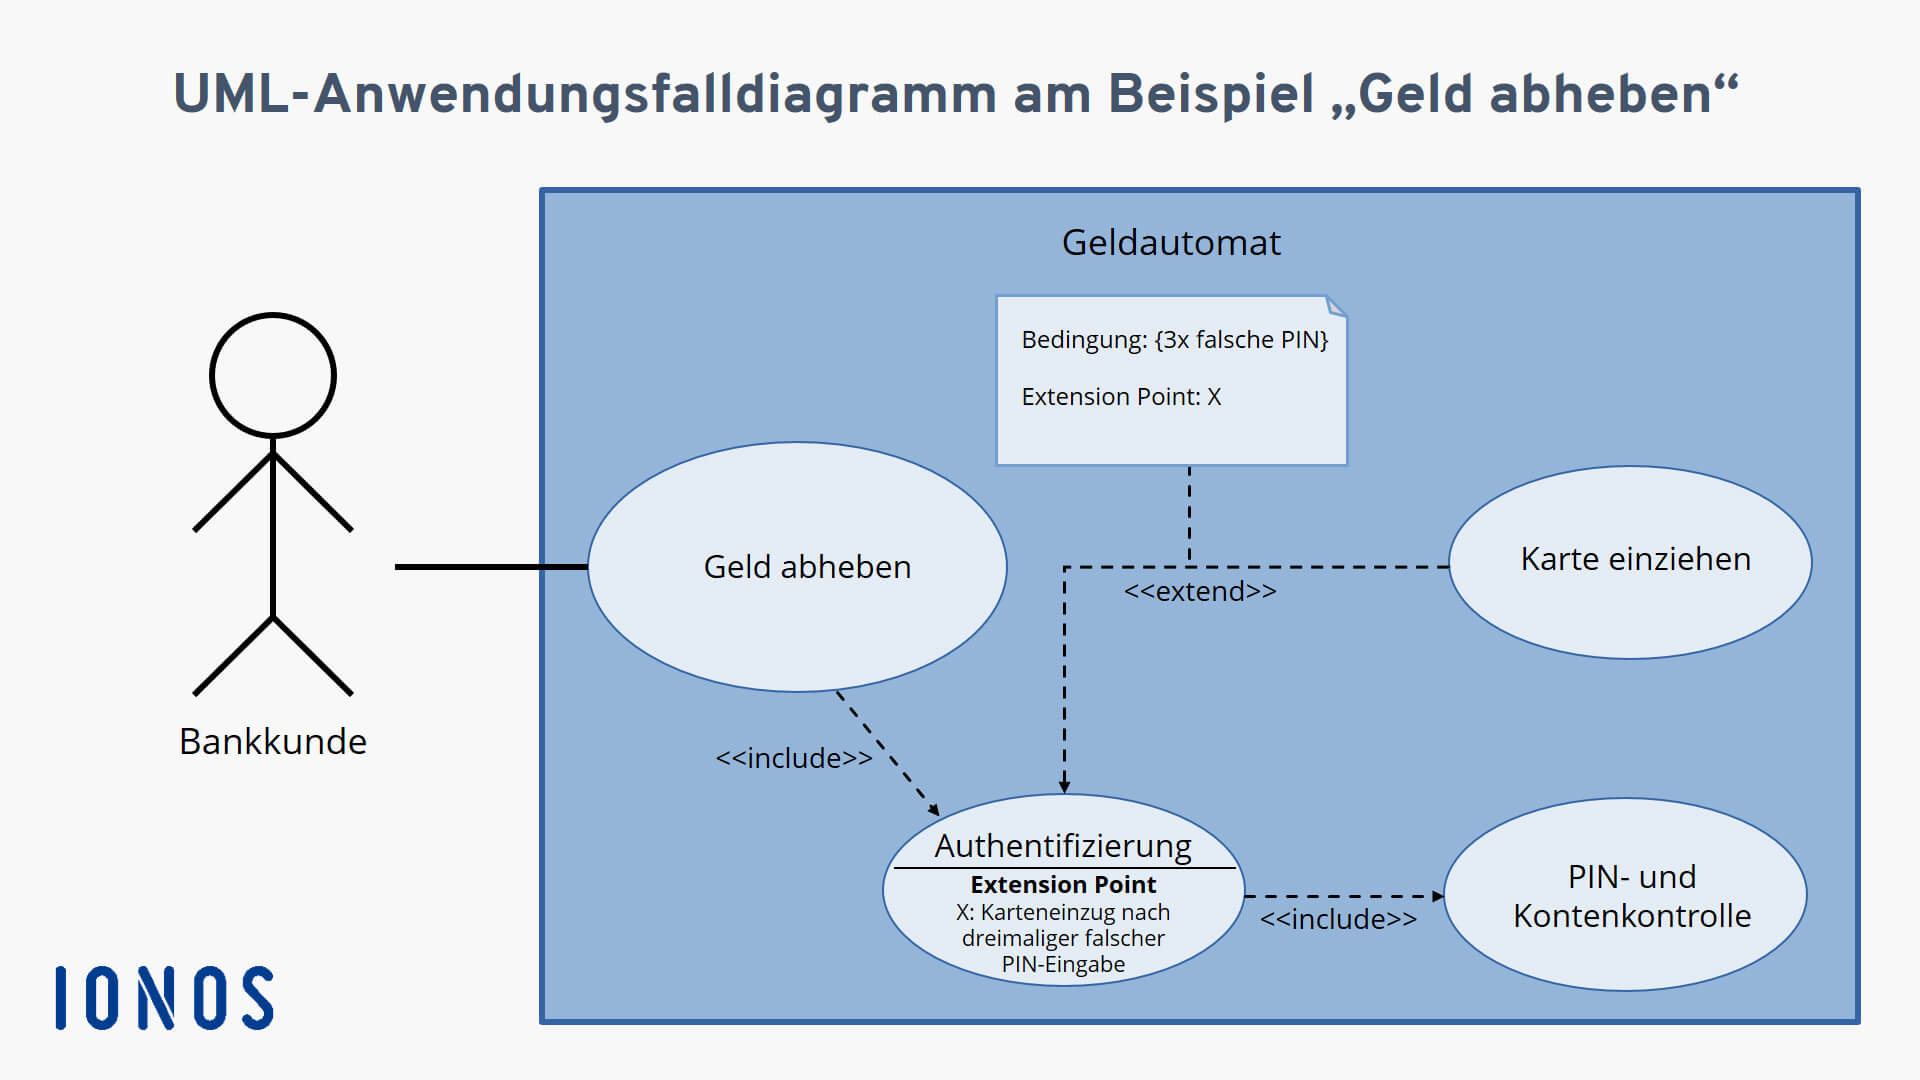
\includegraphics[scale=.25]{Bilder/UseCaseDiagramBeispiel.png}
\end{center}

\subsubsection{Zustandsdiagramm}
\label{sec:Zustandsdiagramm}

\begin{center}
	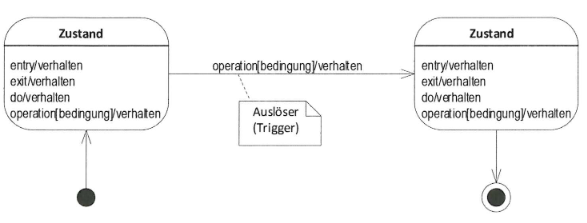
\includegraphics[scale=.9]{Bilder/Zustandsdiagramm.png}
\end{center}

\subsubsection{Aktivitätsdiagramm}
\label{sec:Aktivitaetsdiagramm}

\begin{center}
	\includegraphics[scale=.7]{Bilder/Aktivitätsdiagramm.png}
\end{center}

